\documentclass[11pt, fullpage,letterpaper]{article}

\usepackage[margin=1in]{geometry}
\usepackage{url}
\usepackage{amsmath,amsthm,amssymb}
\usepackage{float}
\usepackage{pgfplots}
\usepgfplotslibrary{polar}
\usepgflibrary{shapes.geometric}
\usetikzlibrary{calc}

\pgfplotsset{my style/.append style={axis x line=middle, axis y line=
middle, xlabel={$x$}, ylabel={$y$}, axis equal }}

\newcommand{\semester}{Fall 2016}
\newcommand{\assignmentId}{4}
\newcommand{\releaseDate}{Oct 18, 2016}
\newcommand{\dueDate}{Nov 1, 2016}

\newcommand{\bx}{{\bf x}}
\newcommand{\bw}{{\bf w}}
\DeclareMathOperator{\sgn}{sgn}

\title{Learning Best Verification Tool for SVCOMP Benchmarks}

\date{CS 6350: Machine Learining \semester\\Intermediate Report}
\author{Group: DABAGHCHIAN \& DAS}

\begin{document}
\pagenumbering{gobble}
\maketitle

\pagebreak
\pagenumbering{arabic}

%parent: main.tex
\section{Introduction}
\label{intro}
The SVCOMP is a competition for software verification tools. There is an established set of verification tasks for comparing software verifiers, and the tools and benchmarks are publicized on the SV-COMP web site. SVCOMP benchmarks are partitioned into different \emph{categories} manually grouped by characteristic features such as usage of \emph{array}, \emph{bitvector}, \emph{concurrency}, and etc. Each category has a bunch of verification tasks which is a C source file \emph{f} and a verification property \emph{p}. The property is either \emph{reachability} or \emph{memory safety}. The designers of these benchmarks have labeled the true property type of each verification task. The competition assigns \emph{score} to each tool's result on a verification task $v$, and normalized sum of such scores of tasks in a category results in the \emph{category score}.

\subsection{Learning Problem}
We are aiming to build a machine learning portfolio solver which given a test verification task, it predicts the tool of choice for verification of this task. To do so, we basically implement the contribution in the paper \cite{DPVF:tool}, and build a linear classifier which trains on the SVCOMP 2014 results. Then, we will use SVCOMP 2015 results as the test data for our classifier. We have already collected and analyzed the required SVCOMP data, and read the reference paper \cite{DPVF:tool} in detail. Also, we have investigated how to implement the target classifier as we will discuss more in the following sections.

\subsection{Program Metrics as Feature Vectors}
We use two sets of program features introduced in \cite{DPVF:tool}: (1) variable role based metrics; (2) loop pattern based metrics. The following is describing each type of metrics in more detail.
\paragraph{Role Based Metrics}
Intuitively, a variable role is the pattern of how a variable is used in a program. For instance, an \emph{integer} variable could be used as a counter in a program, then it has the role COUNTER. Some other examples of roles such as BITVECTOR, LINEAR and etc. can be found in \cite{DPVF:tool, DVZ:var:role}. For a given verification task, the value of each variable feature as the ratio $\frac{|Res^R|}{|Vars|}$ is computed, where $Res^R$ is a mapping from variable roles to the program variable, and $Vars$ is the set of all variables in the given task.
\paragraph{Loop Pattern Based Metrics}
Loops are considered in four patterns as: \emph{syntactically bounded loops} $\mathcal{L}^{SB}$, \emph{syntactically terminating loops} $\mathcal{L}^{ST}$, \emph{simple loops} $\mathcal{L}^{simple}$ and \emph{hard loops} $\mathcal{L}^{hard}$. For a given verification task, the value of each loop feature as the ratio $\frac{|\mathcal{L}^P|}{|Loops|}$ is computed, where $P \in \{ST, SB, simple, hard\}$, and $Loops$ is the set of all loops in the given task.

We extract the above mentioned metrics using the extraction tool from \cite{DPVF:tool} which uses \emph{data flow analysis}. We use the extracted metrics as feature vectors in a manner described below.


%parent: main.tex
\section{Data Organization}
\label{data}
The value of a feature vector depends strongly on the program, and weakly on the category. So, expanding each category to its constituent verification task. Then, we can use this entire set of verification tasks, combined from all the categories, to pursue a stronger classifier than the category based classifier. We use the \emph{category score} to label each verification task corresponding to that category in the training data. Assuming there are two categories of verification tasks, $c_1=\{v^1_1, v^1_2, ..., v^1_{m_1}\}$ and $c_2=\{v^2_1, v^2_2, ..., v^2_{m_2}\}$, where $v^i_j$ denotes the verification task $v_j$ in the category $c_i$. If the $i^{th}$ category has the score $s_i$. For example, if $f=(f_1, f_2, f_3, f_4, f_5)$ is the feature vector, then Table 1 would represent the training data set for all programs in those two categories. 
\begin{table}
\label{tbl:training_data}
\centering
\begin{tabular}{ccc|c|c|c|c||c}
$v$ & & $f_1$ & $f_2$ &  $f_3$ & $f_4$ & $f_5$ & Lable \\
\hline
$v^1_1$ & & $0$ & $0.23$ &  $0.3$ & $0.5$ & $0.1$ & $s_1$ \\
$\dots$ & & $\dots$ & $\dots$ &  $\dots$ & $\dots$ & $\dots$ & $s_1$ \\
$v^1_{m_1}$ & & $0.2$ & $0$ &  $0.1$ & $0.03$ & $0.3$ & $s_1$ \\
$v^2_{1}$ & & $0.1$ & $0.2$ &  $0.05$ & $0.25$ & $0$ & $s_2$ \\
$\dots$ & & $\dots$ & $\dots$ &  $\dots$ & $\dots$ & $\dots$ & $s_2$ \\
$v^2_{m_2}$ & & $0.02$ & $0.07$ &  $0.11$ & $0.3$ & $0.8$ & $s_2$ \\
\end{tabular}
\caption{The training data for two categories $c_1=\{v^1_1, v^1_2, ..., v^1_{m_1}\}$ and $c_2=\{v^2_1, v^2_2, ..., v^2_{m_2}\}$}
\end{table}
According to Table 1, the label of each verification task $v^i_j$ is the score of its corresponding category $c_i$. However SVCOMP results reflect that even though one tool was a winner in a category, there is a possibility that several other tools pose a close performance to the winner. Therefore, we introduce the probabilistic distribution of the scores of the tools on the labels. For example, for $v^1_1$, the label corresponding to a tool $t_k$ would be $\frac{s_k}{\sum \limits_{1 \leq p \leq N} s_p}$, where $s_k$ is the score of $t_k$ for $v^1_1$, and $N$ is the total number of tools. Thus, we get $N$ columns of labels corresponding to each tool. To simplify, we divide the entire training set into $N$ tables, where the label of $k^{th}$ table corresponds to the tool $t_k$ across all the verification tasks. Then, we continue to learn a linear classifier for each tool corresponding to each table. A linear classifier for each tool will be $\sum \limits_{f_i \in \mathcal{F}} val(f_i)w_i$, where $\mathcal{F}$ is the set of all features, $val(f_i)$ denotes the value of that feature, $1 \leq i \leq |\mathcal{F}|$, $w_i \in \mathbb{R}$ and $0 \leq val(f_i) \leq 1$.

%parent: main.tex
\section{Learn the Best Tool}
\label{classification}
In this section we elaborate on how we use Linear Regression classification to learn the best tool for every given verification task.

\subsection{Linear Regression Classifier}
Linear Regression Classifier supports data with real value labels. Therefore, it is a very useful in real world applications. As such, it is very popular, and is used widely. 

%parent: main.tex
\section{Testing and Evaluation}
\label{eval}
We have considered multiple approaches for the Testing and Evaluation phase. A detailed discussion is presented in the following section. 
%\newline
\subsection{Training on full svcomp14 and testing on full svcomp15}
 Svcomp15 had changes in its method of score assignment and evaluation strategies in comparison to svcomp14. Moreover, there were a bunch of new tools, $T_{new}$, that participated in svcomp15 , not present in svcomp14, while there are also a set of tools, $T_{old}$, that participated in 2014 but are absent in 2015. Since we have learnt based on the data of 2014, we only have learned predictors for the set of 2014. Hence, from the 2015 data-set we have curtailed out the new tools, while the old tools that did not participate at all are treated as non-participating, that is, their scoring is set to a low value beyond the minimum normalized score as discussed earlier. This leads to the fact that predictions using the 2014 based learned predictors will not match the svcomp reported results of 2015 over various categories. However, we feel there are two valuable aspects that we can focus on while comparing our predicted results with that of svcomp15. Firstly, how well the $T_{old}$ would have performed if they had participated, and secondly, for tools that participated in both , has there been an improvement in the tool's performance from the previous year? \newline
 For the first question, we get interesting results. 
As shown in the Figure \ref{fig:test_nonlin_15}, LLBMC did participate in svcomp14, but not in svcomp15. That acquired the third rank in svcomp14, and it is expected that it could be ranked as second winner if it had participated. Also, CPAChecker is our predicted winner, that matches with the published results on svcomp15. The tool CBMC came third in svcomp15, whereas our prediction shows it in the forth position closely competing by ESBMC. This slight deviation is expected since we do not consider the runtime of the tools unlike the actual competition. The graphs in the svcomp15 website shows those two tools to be closely competing as well.

 For the latter case as well, we see interesting deviations. In svcomp15 UltimateAutomizer came to be in the second position, however our prediction shows it to be one of the least preferred tools. This is because in svcomp14 it performed poorly compared to other tools, and hence according to our learned predictor, it ranks below most of the tools. That suggests this tool possibly has been improved.
 
\begin{figure}
	\label{fig:test_nonlin_15}
	\centering
	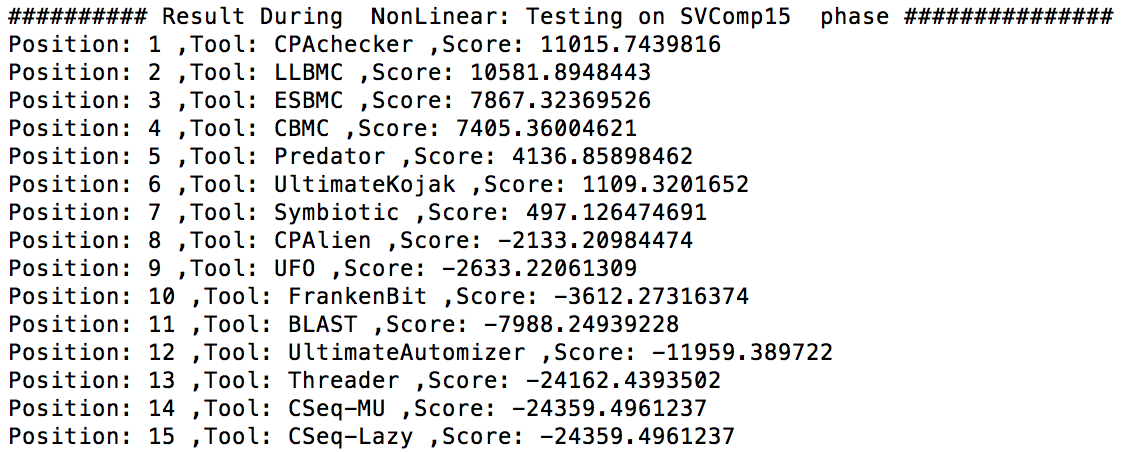
\includegraphics[width = 4.5in]{figures/test15.PNG}
	\caption{Testing on SVComp15 data using learned prediction on SVComp14}
\end{figure} 
 
 %\textbf {NonLinear Regression: With regulariser}
 \subsection{Partitioning SVComp14 as training and test data}
 This is in accordance to the method followed in [1]. Since there is a mismatch in scoring mechanisms between svcomp14 and svcomp15, and also the possible improvements that has been implemented in the participating tools over the year. Hence, in this method we choose svcomp14 as the complete data for both training and testing. To make sure that test data is never seen during the training phase, we perform a randomized split of the data in a $60:40$ ratio(following[1]) such that a random $60\%$ becomes the $train_{14}$ data and the remaining $40\%$ becomes the $test_{14}$ data. Since the partitioning is randomized, we repeat this mechanism 5 times and report the arithmetic mean of the training and test accuracies. In this case as well, we perform cross validation over the regularizer component ($\lambda$) and choose the best one for each tool that determines the final hypothesis for that tool. Since, this is a regression problem, unlike the classification problem of dividing into half-spaces, we have chosen relative error as the measure of accuracy. The relative error is the relative deviations of the predictions from the true score in the test set. The tolerance is chosen to be in $\pm 5\%$ for the reported data. We did try out tighter bounds on accuracy of within $\pm 1\%$, but that gives extremely low accuracy, indicating the fit of the predictor to be within the $5\%$ band of the true score. Our analysis suggest that a looser band is expected since the test label being compared with had an initial approximation of getting the score of its corresponding category and not the exact score it would have had on running over the tools. This we assumed to be a reasonable approximation since benchmarks within a category are expected to resemble closely related feature values and hence should expect similar score. Figure \ref{fig:test_14} shows the accuracy of every tool based on this approach using both basic linear regression and using non-linear transformation with regularization.
 
 \begin{figure}
\centering
\begin{tabular}{c c}
\centering
  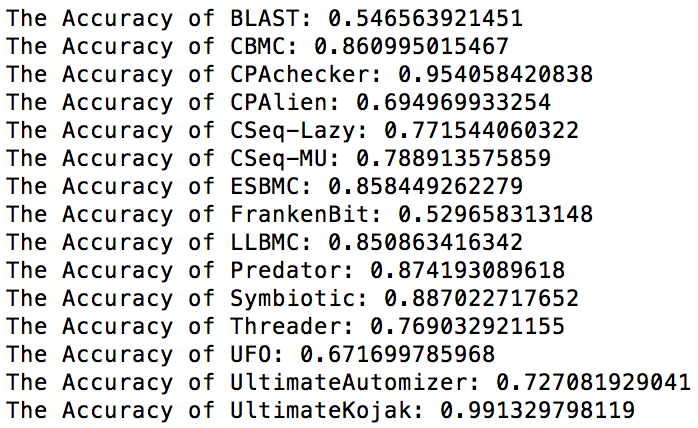
\includegraphics[width=3in]{figures/linear.PNG} &  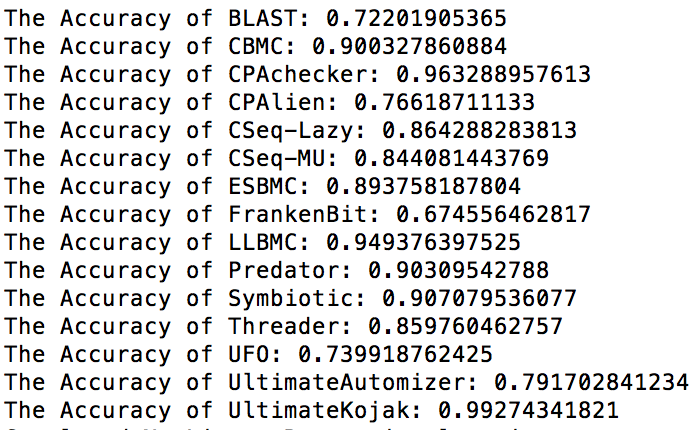
\includegraphics[width=3in]{figures/non_lin.PNG} \\ %
  \small (a) Basic linear regression  \label{fig:sub:lin} & 
  \small (b) Linear regression with non-linear transformation \label{fig:sub:non_lin}
\end{tabular}
\caption{Invariant violation in a virtual wallet example}
\label{fig:test_14}
\end{figure}


%parent: main.tex
\section{Conclusion}
\label{conclusion}



\begin{thebibliography}{9}
\bibitem{DPVF:tool} 
Y. Demyanova, T. Pani, H. Veith, and F. Zuleger.
\textit{Empirical Software Metrics for Benchmarking of Verification Tools}. 
In CAV 2015. LNCS. vol. 9206, pp. 561-579.

\bibitem{DVZ:var:role}
Y. Demyanova, H. Veith, and F. Zuleger.
\textit{On the Concept of Variable Roles and its Use in Software Analysis}.
In Formal Methods in Computer-Aided Design (FMCAD 2013), pp 226-230.
\end{thebibliography}

\end{document}
